\documentclass{article}
\setlength{\parskip}{0pt} % esp. entre parrafos
\setlength{\parindent}{3pt} % esp. al inicio de un parrafo
\usepackage{amsmath} % mates
\usepackage{listings}
\usepackage[sort&compress,numbers]{natbib} % referencias
\usepackage{url} % que las URLs se vean lindos
\usepackage[top=10mm,left=20mm,right=20mm,bottom=25mm]{geometry} % \textbf{\textbf{}}margenes
\usepackage{hyperref} % ligas de URLs
\usepackage{graphicx} % poner figuras
\usepackage{subfigure}
\usepackage[spanish]{babel} % otros idiomas
\hypersetup{
    colorlinks=true,
    linkcolor=blue,
    filecolor=blue,      
    urlcolor=blue,
    citecolor=black,
}

\title{TAREA \# 7 \\ Búsqueda local} %titulo
\author{Natalia Berenice P\'{e}rez L\'{o}pez} % author
\date{\today}

\begin{document} % inicia contenido

\maketitle % cabecera

\section{Objetivo}
El objetivo de esta práctica es crear una visualización (animada) de cómo proceden por lo menos 5 réplicas simultáneas de la búsqueda encima de una gráfica de proyección plana, y después estudiar estadísticamente el efecto que tiene el largo de paso máximo en la cantidad de iteraciones que se requiere para llegar por primera vez al óptimo de la zona de estudio. 

\section{Desarrollo} % seccion y etiqueta
Para generar el código de esta práctica se realizaron algunas ideas y pruebas iniciales, las cuales se encuentran en \href{https://github.com/nataliaperez0/Simulation/tree/main/Tarea7}{mi repositorio}  en GitHub. Se inició tomando como base el código para las réplicas en ejecución paralela en \texttt{Rstudio} \citep{1}. Las modificaciones que se le realizaron al código fueron: variar la función ejemplo y hacerla bidimensional, restringir la función en un intervalo máximo para $x$, $y$, con la técnica del ejemplo unidimensional hacer que los puntos rojos busquen el máximo global de la función en lugar del mínimo, para esto se utilizó apoyo del repositorio de Montemayor \citep{2}, también se agregó un ciclo \texttt{for} para variar el $paso$ con el que se mueven los puntos rojos y otro ciclo \texttt{for} para hacer repeticiones del código y así poder analizar el efecto del $paso$ en un diagrama caja-bigote.
\bigskip

La variante de la función ejemplo bidimensional se muestra en la función \eqref{funcion}.

\begin{equation}
f(x,y) = sin(2x) * ((x + 1)^4 - 30x^2 -50x) + (y + 1)^4 - 30y^2 - 50y
\label{funcion}
\end{equation}

Las restricciones son $ -2 \leq x, y \leq 5 \ $. En la figura \ref{f1} $(a)$ muestra la función \eqref{funcion} graficada en tres dimensiones y $(b)$ muestra una proyección del plano $xy$ donde el valor $z$ se representa con colores.

\begin{figure}[h!]
\centering
\subfigure[Función graficada en 3D.]{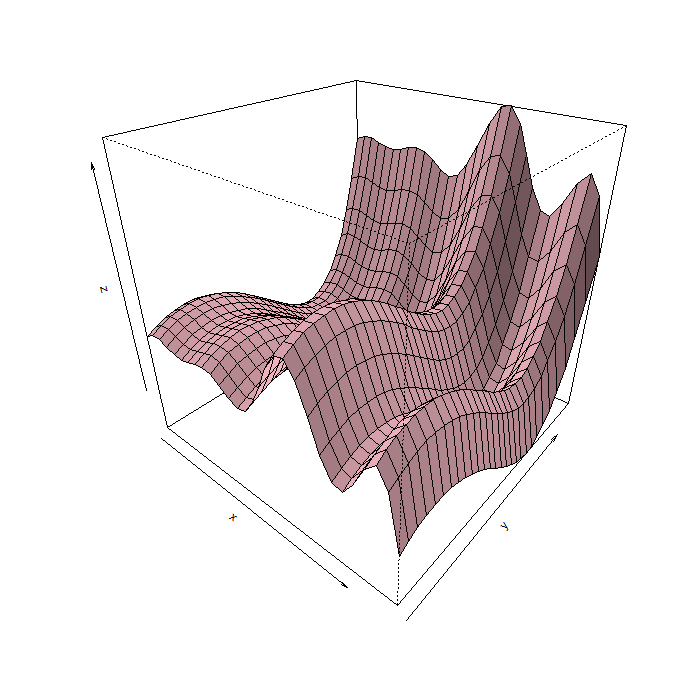
\includegraphics[width=71mm]{Figura1.png}}
\subfigure[Proyección del plano $xy$.]{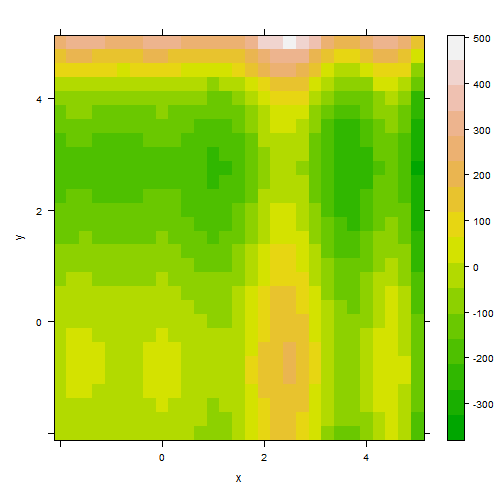
\includegraphics[width=71mm]{Figura2.png}}
\caption{Visualización gráfica de la función \eqref{funcion}.} 
\label{f1}
\end{figure}

\newpage
A continuación se muestra el código para obtener la función bidimensional graficada en 3D: 


\definecolor{verde}{rgb}{0,0.56,0.22}
\definecolor{codegray}{rgb}{0.5,0.5,0.5}
\definecolor{codegreen}{rgb}{0,0.56,0.22}
\definecolor{backcolour}{rgb}{0.95,0.95,0.92}
\definecolor{azul}{rgb}{0,0,1}

\lstdefinestyle{mystyle}{
    backgroundcolor=\color{backcolour},   
    commentstyle=\color{verde},
    keywordstyle=\color{azul},
    numberstyle=\tiny\color{codegray},
    stringstyle=\color{codegreen},
    basicstyle=\ttfamily\footnotesize,
    breakatwhitespace=false,         
    breaklines=true,                 
    captionpos=b,                    
    keepspaces=true,                 
    numbers=left,                    
    numbersep=5pt,                  
    showspaces=false,                
    showstringspaces=false,
    showtabs=false,                  
    tabsize=2
}

\lstset{style=mystyle}
\begin{lstlisting}[language=R, caption= Código graficar la función \eqref{funcion} en 3D.]
g <- function(x,y) {
  return((sin(x*2) * ((x + 1)^4 - 30 * x^2 -50 * x) + (y + 1)^4 - 30 * y^2 - 50 * y))
}
x <- seq(-2, 5, 0.25) 
y <- x
z <- outer(x, y, g)
png("p7_2d.png", width = 700, height = 700)
persp(x, y, z, shade = 0.2, col = 'pink', theta = 40, phi = 30)
graphics.off()
\end{lstlisting}

El código para obtener la proyección del plano $xy$ de la función \eqref{funcion} es el siguiente:

\lstset{style=mystyle}
\begin{lstlisting}[language=R, caption= Código para la proyección del plano $xy$.]
g <- function(x,y) {
  return((sin(x*2) * ((x + 1)^4 - 30 * x^2 -50 * x) + (y + 1)^4 - 30 * y^2 - 50 * y))
}
x <- seq(-2, 5, 0.25) 
y <- x
z <- outer(x, y, g)
dimnames(z) = list(x, y)
library(reshape2)
d = melt(z)
names(d) = c("x", "y", "z")
library(lattice)
png("p7_flat_2.png", width = 500, height = 500)
levelplot(z ~ x * y, data = d, col.regions = terrain.colors(100))
graphics.off()
\end{lstlisting}

Enseguida se muestra el código objetivo de la práctica:

\lstset{style=mystyle}
\begin{lstlisting}[language=R, caption= Código objetivo de la práctica.]
library(lattice)
library(sp)
library(viridisLite)
library(reshape2)
library(ggplot2)
library(tidyverse)
library(ggpubr)
library(car)
library(rstatix)
library(rapportools)
library(readr)
library(gridExtra)

g <- function(x,y) {
  return((sin(x*2) * ((x + 1)^4 - 30 * x^2 -50 * x) + (y + 1)^4 - 30 * y^2 - 50 * y))
}

x <- seq(-2, 5, 0.25) 
y <- x
z <- outer(x, y, g)

low <- -2
high <- 5
pasos <- seq(0.25, 2, 0.25) #variar el paso
replicas <- 50 #cantidad de puntos rojos
df<- data.frame()

for (step in pasos) {
  for (repetir in 1:30){ #hacer repeticiones del experimento
    replica <- function(t) {
      curr <- c(runif(1, low, high), runif(1, low, high))
      best <- curr
      for (tiempo in 1:t) {
        delta <- runif(1, 0, step)
        izq <- curr +c(-delta,0)
        der <- curr + c(delta,0)
        arr <- curr + c(0,-delta)
        aba <- curr + c(0,delta)
        
        coord <- c(izq, der, arr, aba)
        for(p in 1:8){
          if(coord[p] < (-2)){
            coord[p] <- coord[p]+5
          }
          if(coord[p] > 5){
            coord[p] <- coord[p]-2
          }
        }
        
        vx<-c()
        vy<-c()
        for(q in 1:8){
          if(q %% 2 == 0){
            vy <- c(vy,coord[q])
          }else{
            vx <- c(vx,coord[q])
          }
        }
        
        vg<- c()
        for(k in 1:4){
          vg <- c(vg, g(vx[k], vy[k]) )
        }
        
        pmax <- which.max(vg)
        curr <- c(vx[pmax], vy[pmax])
        if(g(curr[1],curr[2]) > g(best[1],best[2])){
          best <- curr
        }
      }
      return(best)
    }
    
    suppressMessages(library(doParallel))
    registerDoParallel(makeCluster(detectCores(logical = FALSE) - 2))
    
    for (pot in 1:40) { #iteraciones
      tmax <- pot
      resultados <- foreach(i = 1:replicas, .combine=c) %dopar% replica(tmax)
      
      vx<- c()
      vy<- c()
      aux<-(2*replicas)
      for(q in 1:aux){
        if(q %% 2 == 0){
          vy <- c(vy,resultados[q])
        }else{
          vx <- c(vx,resultados[q])
        }
      }
      
      val <- c()
      for(k in 1:replicas){
        val <- c(val, g(vx[k], vy[k]))
      }
      
      maximo <- which.max(val)
      x <- seq(-2, 5, 0.25) 
      y <-  x
      z <- outer(x, y, g)
      dimnames(z) <- list(x, y)
      d <- melt(z)
      names(d) <- c("x", "y", "z")
      
      if (repetir == 1 & step == 0.25){
        png(paste0("t7_", tmax, ".png", sep=""), width=500, height=500)
        plot(levelplot(z ~ x * y, data = d, col.regions = terrain.colors(100)))
        trellis.focus("panel", 1, 1, highlight=FALSE)
        lpoints(vx, vy, pch=20, col="red", cex=2) #puntos rojos
        trellis.unfocus()
        trellis.focus("panel"[1], 1, 1, highlight=FALSE) 
        lpoints(vx[maximo], vy[maximo], pch=20, col="blue",cex=3) #raya azul
        trellis.unfocus()
        graphics.off()
      }
    }
    ultimo<-min(val)
    df<- rbind(df,c(step,repetir,ultimo))
  }
}
stopImplicitCluster()

#GRAFICAR
names(df) <- c("Paso", "Repeticion", "Minimo")
df$Paso = as.factor(df$Paso)
ggplot(df, aes(x= Paso, y= Minimo, fill= Paso)) + 
  geom_boxplot()+
  labs(x = "Paso", y = "Valor minimo")
\end{lstlisting}

Con el código anterior los $50$ puntos rojos buscan alcanzar el punto máximo de la función bidimensional \eqref{funcion}, además se varía el $paso$ de los puntos rojos en valores de 0.25, 0.5, 0.75, 1, 1.25, 1.5. 1.75 y 2, para cada $paso$ se hacen $30$ repeticiones del exprimento lo cual permite analizar con que $paso$ los puntos rojos llegan con más éxito al máximo de la función. 
\bigskip

La figura \ref{f2} muestra los resultados obtenidos con un $paso = 0.25$, se pueden ver los $50$ puntos rojos y un punto azul que indica el valor máximo al que han llegado los puntos rojos en las $40$ iteraciones.

\begin{figure}[h!]
\centering
\subfigure[Paso 1.]{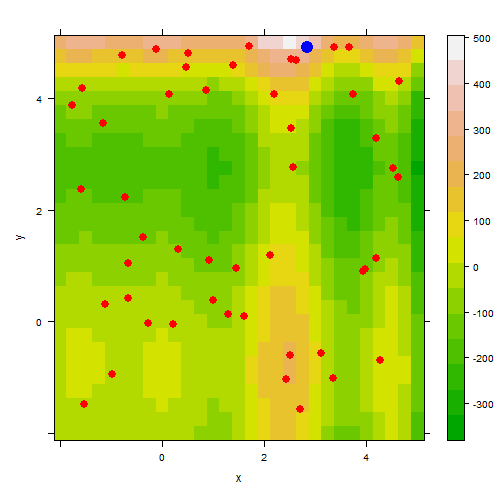
\includegraphics[width=60mm]{t7_1.png}}
\subfigure[Paso 10.]{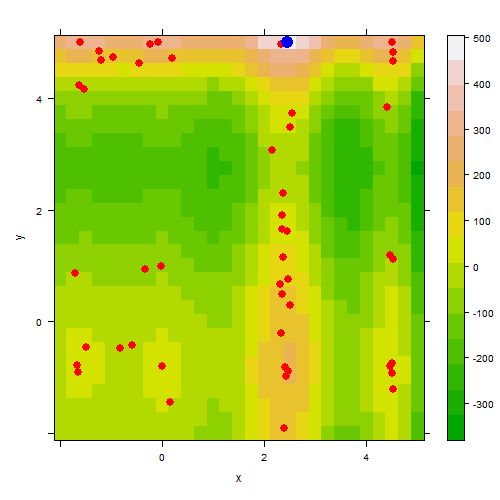
\includegraphics[width=60mm]{t7_10.png}}
\subfigure[Paso 20.]{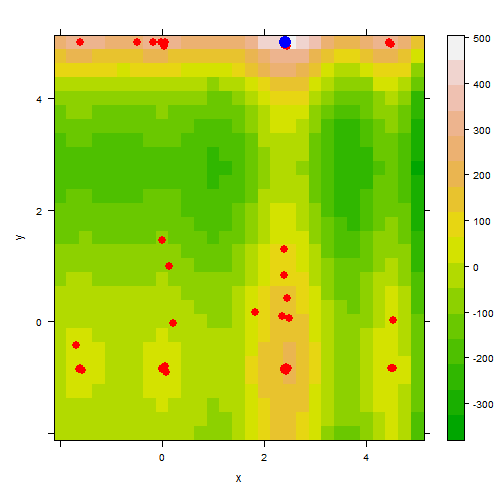
\includegraphics[width=60mm]{t7_20.png}}
\subfigure[Paso 40.]{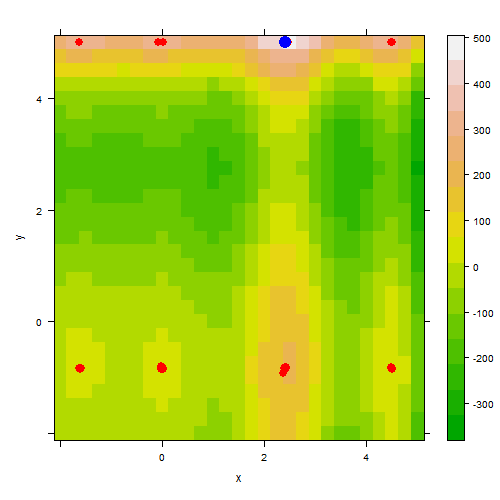
\includegraphics[width=60mm]{t7_40.png}}
\caption{Búsqueda local de la función \eqref{funcion} con un $paso = 0.25$.} 
\label{f2}
\end{figure}

En la figura \ref{f3} se muestran los resultados obtenidos con un $paso = 2$.

\begin{figure}[h!]
\centering
\subfigure[Paso 1.]{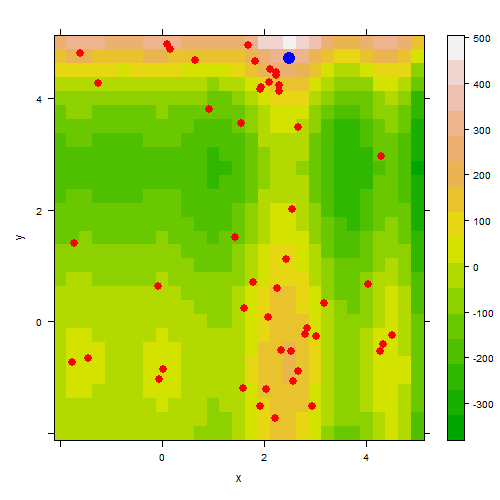
\includegraphics[width=60mm]{t7_1_2.png}}
\subfigure[Paso 10.]{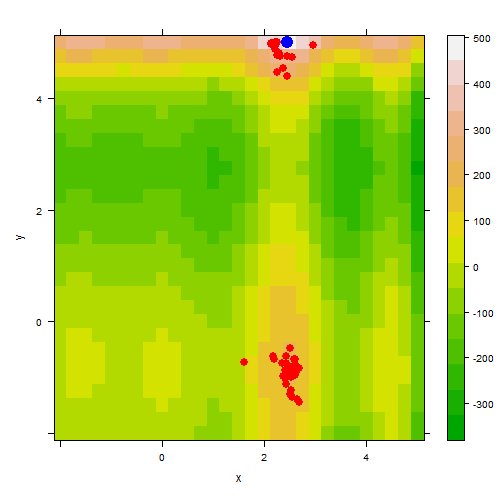
\includegraphics[width=60mm]{t7_10_2.png}}
\subfigure[Paso 20.]{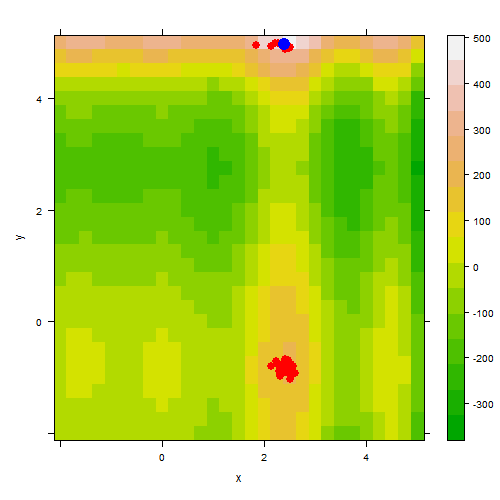
\includegraphics[width=60mm]{t7_20_2.png}}
\subfigure[Paso 40.]{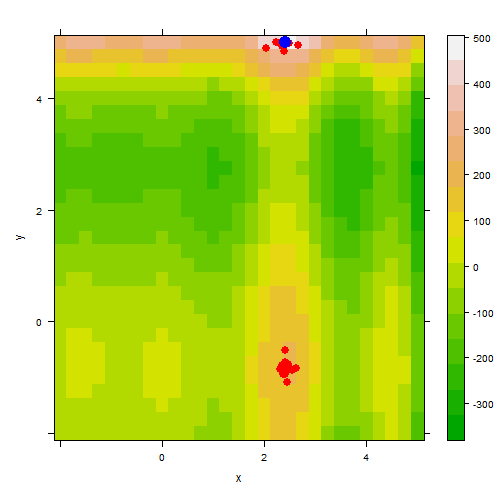
\includegraphics[width=60mm]{t7_40_2.png}}
\caption{Búsqueda local de la función \eqref{funcion} con un $paso = 2$.} 
\label{f3}
\end{figure}

Los gifs \citep{4} de las búsquedas locales de cada $paso$ se encuentran \href{https://github.com/nataliaperez0/Simulation/tree/main/Tarea7}{mi repositorio} en GitHub.
\bigskip

En la figura \ref{f3}, la cual tiene un $paso$ de $2$, se puede ver que una mayor cantidad de puntos rojos lograr alcanzar el punto máximo de la función bidimensional, mientras que con un $paso$ de $0.25$ (ver figura \ref{f2}) varios puntos rojos se quedan en zonas más bajas de la función.
\bigskip

Para analizar visualmente el valor mínimo al que llegan los puntos rojos con cada $paso$ se realizó un diagrama caja-bigote con las $30$ replicas del exprimento para cada $paso$ (ver figura \ref{f4}). En el diagrama podemos observar que con pasos grandes como $1.5$, $1.75$ y $2$ los puntos rojos que no logran llegar al punto máximo de la función (punto azul), si logran llegar a zonas altas.
\bigskip

Para analizar si existe una relación entre la variación del $paso$ y qué tan alto pueden llegar los puntos rojos que no logran llegar al punto máximo de la función \eqref{funcion} se realizó una prueba estadística. Primero se elegió utilizar la prueba estadística ANOVA de una vía, pero debido a los resultados obtenidos al revisar la normalidad de los datos, se eligió realizar la prueba estadística \texttt{Kruskal Wallis}.
\bigskip

En el cuadro \ref{Cuadro1} se  resumen los resultados de la revisión de los supuestos para poder aplicar la prueba estadística. El supuesto outliers se refiere a la cantidad de valores atípicos que existen en los grupos, la normalidad por grupos se obtuvo con la prueba de \texttt{Shapiro Wilk} y la homogeneidad de varianza se obtuvo con la prueba de \texttt{Levene}.

\newpage
.
\bigskip

\begin{figure} [h!]% figura
    \centering
    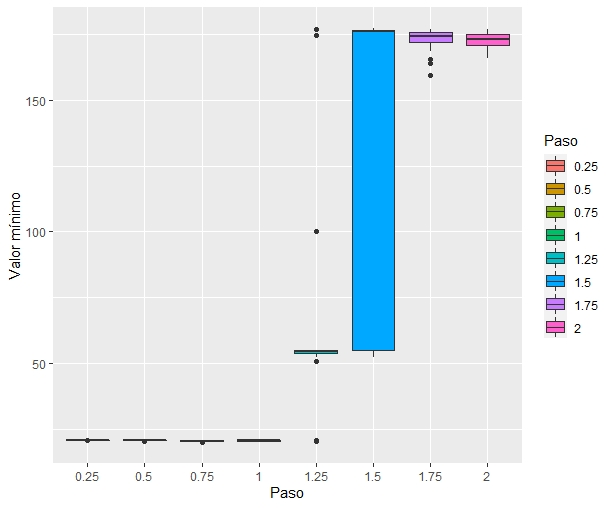
\includegraphics[width=150mm]{Figura12.jpeg} % archivo
    \caption{Valor mínimo al que llegan los puntos rojos en cada $paso$.}
    \label{f4}
\end{figure}

\begin{table}[ht]
\centering
\caption{Resultados del los supuestos para aplicar la prueba estadística.}
\smallskip

\begin{tabular}{ |p{2.1cm}|p{13cm}|}
 \hline
 Outliers & $14$ \\
 \hline
 Normalidad por grupo & $0.25$: $p$ = $0.004$ / $0.50$: $p$ = $0.106$ / $0.75$: $p$ = $0.010$ / $1$: $p$ = $0.061$ / $1.25$: $p$ = $1.05\times 10^{-8}$  $1.5$: $p$ = $1.68\times 10^{-7}$ / $1.75$: $p$ = $7.72\times 10^{-5}$ / $2$: $p$ = $0.122$ \\
 \hline
 Homogeneidad de varianza & $p$ = $1.18\times 10^{-11}$ \\
 \hline
\end{tabular}
\label{Cuadro1}
\end{table}

En los resultados se observa que para la normalidad por grupos existen valores de $p$ menores a $0.05$, por lo tanto no se tiene normalidad, así que es necesario realizar la prueba estadística \texttt{Kruskal Wallis}.
\bigskip

Al realizar la prueba \texttt{Kruskal Wallis} se obtienen los resultados mostrados en el cuadro \ref{Cuadro2}.

\begin{table}[h!]
\centering
\caption{Resultados al aplicar la prueba estadística \texttt{Kruskal Wallis}.}
\smallskip

\begin{tabular}{ |p{2.1cm}|p{2.1cm}|}
 \hline
 Chi cuadrada & Valor de $p$ \\
 \hline
 $197.35$ & $2.2\times 10^{-16}$ \\
 \hline
\end{tabular}
\label{Cuadro2}
\end{table}

Hipótesis nula : Las medias son iguales en todos los grupos.
\smallskip

Hipótesis alternativa: Debido a que $p < 0.05$ se rechaza la hipótesis nula, es decir que si existen diferencias significativas entre las medias de los grupos. 
\smallskip

\newpage
.
\bigskip

Se entiende entonces que la variación del $paso$ en el movimiento de los puntos rojos si tiene un efecto significativo en qué tan alto logran llegar en la función bidimensional.
\bigskip

También podemos realizar la prueba de suma de rangos de \texttt{Wilcoxon} por pares \citep{3} para observar los resultados de $p$ y determinar si existen diferencias al comparar entre ellos los pasos (Ver cuadro \ref{Cuadro3}).

\begin{table}[ht]
\centering
\caption{Resultados al aplicar la prueba \texttt{Wilcoxon}.}
\smallskip

\begin{tabular}{|p{1.7cm}|p{1.7cm}|p{1.7cm}|p{1.7cm}|p{1.7cm}|p{1.7cm}|p{1cm}|p{1cm}|}
 \hline
Valor de $p$ & $0.25$ & $0.50$ & $0.75$ & $1.0$ & $1.25$ & $1.50$ & $1.75$\\
 \hline
 $0.50$ & $1.1\times 10^{-5}$ & - & - & - & - & - & - \\
 \hline
 $0.75$ & $4.7\times 10^{-12}$ & $1.6\times 10^{-5}$ & - & - & - & - & - \\
 \hline
 $1.0$ & $0.0005$ & $0.7487$ & $0.5131$ & - & - & - & - \\
 \hline
 $1.25$ & $5.5\times 10^{-9}$ & $8.2\times 10^{-11}$ & $4\times 10^{-12}$ & $3.5\times 10^{-11}$ & - & - & - \\
 \hline
 $1.50$ & $4.7\times 10^{-16}$ & $4.7\times 10^{-16}$ & $4.7\times 10^{-16}$ & $4.7\times 10^{-16}$ & $2.2\times 10^{-5}$ & - & - \\
 \hline
 $1.75$ & $4.7\times 10^{-16}$ & $4.7\times 10^{-16}$ & $4.7\times 10^{-16}$ & $4.7\times 10^{-16}$ & $1.3\times 10^{-10}$ & $1$ & - \\
 \hline
 $2.0$ & $4.7\times 10^{-16}$ & $4.7\times 10^{-16}$ & $4.7\times 10^{-16}$ & $4.7\times 10^{-16}$ & $1.7\times 10^{-10}$ & $1$ & $1$ \\
 \hline
\end{tabular}
\label{Cuadro3}
\end{table}

En los resultados de la prueba podemos observar que la mayoría de los valores de $p$ son menores a $0.05$, solo existen algunas excepciones en las cuales se tiene una $p > 0.05$ como por ejemplo en la $paso = 1$ comparada con la $paso = 0.5$, lo cual indica que entre ellas no existen diferencias significativas en sus medias.
\bigskip

A continuación se muestra el código utilizado para realizar la prueba estadística \texttt{Kruskal Wallis}:

\lstset{style=mystyle}
\begin{lstlisting}[language=R, caption= Código para las pruebas estadísticas \texttt{Kruskal Wallis} y \texttt{Wilcoxon}.]
library(tidyverse)
library(ggpubr)
library(rstatix)
library(rapportools)
library(readr)

#Estadisticas descriptivas
df %>%
  group_by(Paso) %>%
  get_summary_stats(Minimo, type = "mean_sd")

#SUPUESTOS PARA ANOVA
#1:Outliers
df %>%
  group_by(Paso) %>%
  identify_outliers(Minimo)

#2:Normalidad por Shapiro
df %>%
  group_by(Paso) %>%
  shapiro_test(Minimo)

#3:Homogeneidad de varianza con prueba Levene
df %>%
  levene_test(Minimo~Paso)

#PRUEBA ESTADISTICA KRUSKAL WALLIS
kruskal.test(Minimo ~ Paso, data = df)

#PRUEBA WILCOXON
pairwise.wilcox.test(df$Minimo, df$Paso)
\end{lstlisting}

\newpage
.
\bigskip

\section{Conclusi\'{o}n}
Con base en las gráficas de las iteraciones de cada $paso$, el diagrama caja-bigote y los resultados obtenidos de las pruebas estadísticas \texttt{Kruskal Wallis} y \texttt{Wilcoxon} puedo concluir que la variación del $paso$ con que se mueven los puntos rojos si afecta significativamente el valor mínimo que alcanzarán los puntos rojos que no llegan al máximo de la función bidimensional, además se oberva que que a mayor $paso$ más rápidamente llegan los puntos rojos al máximo de la función (punto azul). 
\smallskip

En general en ésta práctica se me dificultó realizar el código y entender el propósito de la prueba estadística, sin embargo con el apoyo de mis compañeros logré realizarla. 
\newpage
.
\bigskip

\bibliography{referencias}
\bibliographystyle{plainnat}

\end{document}